              
% --------------------------------------------------------------
% This is all preamble stuff that you don't have to worry about.
% Head down to where it says "Start here"
% --------------------------------------------------------------
 
\documentclass[12pt]{article}
 
\usepackage[margin=1in]{geometry} 
\usepackage{amsmath,amsthm,amssymb}
\usepackage{hyperref}
\setlength{\parindent}{2em}
\setlength{\parskip}{1em}
\usepackage{graphicx}
%%%%%%%%%%%%%%%%%%%%%%%%
\usepackage{listings}
\usepackage{color}
\usepackage{rotating}

\definecolor{codegreen}{rgb}{0,0.6,0}
\definecolor{codegray}{rgb}{0.5,0.5,0.5}
\definecolor{codepurple}{rgb}{0.58,0,0.82}
\definecolor{backcolour}{rgb}{0.95,0.95,0.92}

\lstdefinestyle{mystyle}{
	backgroundcolor=\color{backcolour},   
	commentstyle=\color{codegreen},
	keywordstyle=\color{magenta},
	numberstyle=\tiny\color{codegray},
	stringstyle=\color{codepurple},
	basicstyle=\footnotesize,
	breakatwhitespace=false,         
	breaklines=true,                 
	captionpos=b,                    
	keepspaces=true,                 
	numbers=left,                    
	numbersep=5pt,                  
	showspaces=false,                
	showstringspaces=false,
	showtabs=false,                  
	tabsize=2
}

\lstset{style=mystyle}
%%%%%%%%%%%%%%%%%%%%%%%%%%%%%%%%%%%%%
\newcommand{\N}{\mathbb{N}}
\newcommand{\Z}{\mathbb{Z}}
 
\newenvironment{problem}[2][Problem]{\begin{trivlist}
		\item[\hskip \labelsep {\bfseries #1}\hskip \labelsep {\bfseries #2.}]}{\end{trivlist}}
\newenvironment{solution}[2][Solution]{\begin{trivlist}
		\item[\hskip \labelsep {\bfseries #1}\hskip \labelsep {\bfseries #2.}]}{\end{trivlist}}
\newenvironment{theorem}[2][Theorem]{\begin{trivlist}
\item[\hskip \labelsep {\bfseries #1}\hskip \labelsep {\bfseries #2.}]}{\end{trivlist}}
\newenvironment{lemma}[2][Lemma]{\begin{trivlist}
\item[\hskip \labelsep {\bfseries #1}\hskip \labelsep {\bfseries #2.}]}{\end{trivlist}}
\newenvironment{exercise}[2][Exercise]{\begin{trivlist}
\item[\hskip \labelsep {\bfseries #1}\hskip \labelsep {\bfseries #2.}]}{\end{trivlist}}
\newenvironment{reflection}[2][Reflection]{\begin{trivlist}
\item[\hskip \labelsep {\bfseries #1}\hskip \labelsep {\bfseries #2.}]}{\end{trivlist}}
\newenvironment{proposition}[2][Proposition]{\begin{trivlist}
\item[\hskip \labelsep {\bfseries #1}\hskip \labelsep {\bfseries #2.}]}{\end{trivlist}}
\newenvironment{corollary}[2][Corollary]{\begin{trivlist}
\item[\hskip \labelsep {\bfseries #1}\hskip \labelsep {\bfseries #2.}]}{\end{trivlist}}
 
\begin{document}
 
% --------------------------------------------------------------
%                         Start here
% --------------------------------------------------------------
 
%\renewcommand{\qedsymbol}{\filledbox}
 
\title{Final Project}%replace X with the appropriate number
\author{Sebastian Gomez-Cardona\\ %replace with your name
622 Computational Economics} %if necessary, replace with your course title
 
\maketitle

In this document I will replicate most of the paper "Income and wealth distribution in macroeconomics: a continuous-time approach" by Achdou et al. This papers has basic algorithms to solve heterogeneous agents models in continuous time. I will focus in 3 parts: i) a Huggett economy, for which I calculate the policy functions and the equilibrium interest rate, ii) MIT shocks in the context of the Huggett model, and iii) the Huggett model including housing, which introduces non-convexities.\\
This document is organize as follows: first I introduce the problem of an agent in the Huggett economy, then I describe the way to solve it based on the viscosity solution for partial differential equations. Third I present the results and an interpretation of them. Finally, I briefly describe the economy with two goods: bonds and housing, and present my results for this model.\\

\section{Huggett model in continuous time}
The economy is populated with a continium of individuals of measure 1. Each individual is infinitely lived, receives income $y_t$, can save in a risk-free asset and has a borrowing constraint of $\underline{a}$. Therefore, we can write
\begin{equation}\label{eq1}
\begin{split}
&\max_{c_t, t\geq 0} E_0 \int_0^\infty e^{-\rho t} u(c_t) dt\\
&\text{s.t.      } \dot{a}_t=y_t+r_t a_t-c_t \\
&a_t\geq \underline{a}
\end{split}
\end{equation}

If we assume that there are only two possible values for the income shock, $y_1, y_2$, then we can denote $g_j(a,t)$ as the pdf of the distribution of agents with wealth $a$ and income $y_j$ at time t. Therefore, the market clearing condition for this economy is (I have assumed that asset is in zero external supply):
\begin{equation}
\int_{\underline{a}}^{\infty}a g_1(a,t)da+\int_{\underline{a}}^{\infty}a g_2(a,t)da=0 \text{   } \forall t
\end{equation}

\section{Derivation of the HJB and KF equations}
For a period of length $\Delta$ individuals discount factor is $e^{-\rho\Delta}$, individuals with income $y_j$ have probability $e^{-\lambda_j\Delta}$ to keep the same income. With this, we can write the Bellman equation for problem \ref{eq1} as
\begin{equation}\label{eqBellman}
\begin{split}
&v_j(a_t)=\max_{c} u(c)\Delta+e^{-\rho\Delta}(e^{-\lambda_j\Delta} v_j(a_{t+\Delta})+(1-e^{-\lambda_j\Delta} )v_{-j}(a_{t+\Delta}))\\
&a_{t+\Delta}=\Delta(y_j+ra_t-c)+a_t\\
&a_{t+\Delta}\geq \underline{a}
\end{split}
\end{equation}
Since we'll make $\Delta\rightarrow 0$ then $e^{-\rho\Delta}\approx 1-\rho\Delta$ and $e^{-\lambda_j\Delta}\approx1-\lambda_j\Delta$. Substituting these in the problem defined in \ref{eqBellman}, and substracting $(1-\rho\Delta)v_j(a)$ from both sides of the objective function, we get
\begin{equation}\label{eqBellman2}
\begin{split}
&\Delta\rho v_j(a_t)=\max_{c} u(c)\Delta+(1-\rho\Delta)( v_j(a_{t+\Delta})-v_j(a_t)+(\Delta\lambda_j)(v_{-j}(a_{t+\Delta})-v_{j}(a_{t+\Delta}))\\
&a_{t+\Delta}=\Delta(y_j+ra_t-c)+a_t\\
&a_{t+\Delta}\geq \underline{a}
\end{split}
\end{equation}
Finally, since
\begin{equation}
\lim_{\Delta\rightarrow0}\frac{v_j(a_{t+\Delta})-v_j(a_t)}{\Delta}=\lim_{\Delta\rightarrow0}\frac{v_j(\Delta(y_j+ra_t-c)+a_t)-v_j(a_t)}{\Delta}=v'_j(a_t)(y_j+ra_t-c)
\end{equation}
dividing \ref{eqBellman2} by $\Delta$ and taking $\Delta\rightarrow0$ we get the HJB equation
\begin{equation}\label{eqHJB}
\rho v_j(a_t)=\max_{c} u(c)+v'_j(a_t)(y_j+ra_t-c)+\lambda_j(v_{-j}(a_{t})-v_{j}(a_{t}))
\end{equation}
Now, before dealing with the boundary condition let's define consumption and savings as derived from the problem above
\begin{equation}\label{eqS}
s_j(a_t)=y_j+ra_t-c_j(a_t)
\end{equation}
\begin{equation}\label{eqC}
c_j(a_t)=(u')^{-1}(v'_j(a_t))
\end{equation}
Now, the borrowing constraint never binds for $a>\underline{a}$ since being above the borrowing constraint at any point in time implies that the agent will also be above it in the immediate future. Now, when $a=\underline{a}$, the boundary condition implies that $s_j(\underline{a})=y_j+r\underline{a}_t-c_j(\underline{a})\geq0$ and the first order condition $u'(c_j(a_t))=v'_j(a_t)$ still holds so $v'_j(a_t)=u'(c_j(a_t))\geq u'(y_j+r\underline{a}_t)$. Therefore, the boundary condition is equivalent to
\begin{equation}\label{eqBoundary}
v'_j(a_t)\geq u'(y_j+r\underline{a}_t)
\end{equation}

Now, in order to derive the KF equation we analyze the evolution of wealth. For any individual the individual wealth evolves according to
\begin{equation}
a_t=a_{t+\Delta}-\Delta s_j(a_{t+\Delta})
\end{equation}
And define the CDF $G_j(a,t)=Pr(a_t\leq a,y_t=y_j)$, which satisfies $G_1(\underline{a},t)+G_2(\underline{a},t)=0$ and $\lim_{a\rightarrow a}(G_1(a,t)+G_2(a,t))=1$, and has densities $g_j(a,t)=\partial_a G_j(a,t)$. \\
Now, assume that for the level of wealth consider agents decumulate assets $s_j(a)\leq0$ (the case for accumulating wealth is symmetric), and that agents don't switch income, therefore
\begin{equation}
Pr(a_{t+\Delta}\leq a)=Pr(a_{t}\leq a)+Pr(a\leq a_{t}\leq a-\Delta s_j(a))=Pr(a_{t}\leq  a-\Delta s_j(a))
\end{equation}
where the first term in the equation above represents those agents already belowe $a$ and the second term represents the agents that crossed the threshold from $t$ to $t+\Delta$. Now, taking into account that agents can switch income
\begin{equation}
\begin{split}
&Pr(a_{t+\Delta}\leq a,t_{t+\Delta}=y_j)\\
&=(1-\Delta\lambda_j)Pr(a_{t}\leq  a-\Delta s_j(a),y_t=y_j)+\Delta\lambda_{-j} Pr(a_{t}\leq  a-\Delta s_j(a),y_t=y_{-j})
\end{split}
\end{equation}
Using the definition of $G(.,.)$, substracting $G_j(a,t)$ from both sides, dividing by $\Delta$ and taking $\Delta \rightarrow 0$
\begin{equation}
\partial_tG_j(a,t)=-s_j(a)\partial_aG_j(a,t)-\delta_jG_j(a,t)+\delta_{-j}G_{-j}(a,t)
\end{equation}
Taking derivatves in both sides with respect to $a$ we get the KF equation
\begin{equation}\label{eqKF}
\partial_tg_j(a,t)=-\partial_a[s_j(a) g_j(a,t)]-\delta_jg_j(a,t)+\delta_{-j}g_{-j}(a,t)
\end{equation}
 
Equations \ref{eqHJB}, \ref{eqS}, \ref{eqC}, \ref{eqBoundary} and \ref{eqKF} fully characterize equilibrium. In a stationary equilibrium the LHS of equation \ref{eqKF} is set to zero (the distribution doesn't change with time) and the rest of equations remain the same

\section{Numerical solution}
In order to solve the HJB equation a finite difference approached is used. An interval in variable $a$ is partitioned and the policy and value functions are approximated in those points (denote the points $a_i$ so that we define $v_{i,j}\equiv v_j(a_i)$). The value function can then be approximated iterating the following equation (which is the HJB equation in \ref{eqHJB})
\begin{equation}\label{eqHJBapp}
\frac{v_{i,j}^{n+1}-v_{i,j}^{n}}{\Delta}+\rho v_{i,j}^{n+1}=u(c_{i,j}^{n})+(v_{i,j}^{n+1})'(z_j+ra_i-c_{i,j}^{n})+\lambda_j(v_{i,-j}^{n+1}-v_{i,j}^{n+1})
\end{equation}
This is an implicit method because equation \ref{eqHJBapp} defines $v_{i,j}^{n+1}$ implicitly. Consumption is defined according to equation \ref{eqC} ($c_{i,j}^n=(u')^{-1}[(v_{i,j}^n)']$). Now, in order to approximate ${v'}_{i,j}^n$ we use a finite difference method, so we define the Forward and Backward difference approximation as
\begin{equation}
v'_{i,j,F}\equiv \frac{v_{i+1,j}-v_{i,j}}{\Delta a}\approx v'_j(a_i)
\end{equation}
\begin{equation}
v'_{i,j,B}\equiv \frac{v_{i-1,j}-v_{i,j}}{\Delta a}\approx v'_j(a_i)
\end{equation}
And the respective definition for savings as
\begin{equation}
s_{i,j,F}=z_j+ra_i-(u')^{-1}(v'_{i,j,F})
\end{equation}
\begin{equation}
s_{i,j,B}=z_j+ra_i-(u')^{-1}(v'_{i,j,B})
\end{equation}
We use one or the other approximation of ($v'(.)$) depending on the sign of the state variable, that is
\begin{equation}
v'_{i,j}=v'_{i,j,F} \bold{1}_{s_{i,j,F}>0}+v'_{i,j,B} \bold{1}_{s_{i,j,F}<0}+\bar{v}'_{i,j} \bold{1}_{s_{i,j,F}\leq0\leq s_{i,j,B}}
\end{equation}
where $\bar{v}'_{i,j}=u'(z_j+ra_i)$. So we can define, for any variable x, $x^{+}=max{x,0}$ and $x^{-}=min{x,0}$. This allows us to write equation \ref{eqHJBapp} as
\begin{equation}\label{eqHJBapp2}
\frac{v_{i,j}^{n+1}-v_{i,j}^{n}}{\Delta}+\rho v_{i,j}^{n+1}=u(c_{i,j}^{n})+\frac{v_{i+1,j}^{n+1}-v_{i,j}^{n+1}}{\Delta a}(s_{i,j,F}^n)^{+}+\frac{v_{i,j}^{n+1}-v_{i-1,j}^{n+1}}{\Delta a}(s_{i,j,B}^n)^{-}+\lambda_j(v_{i,-j}^{n+1}-v_{i,j}^{n+1})
\end{equation}
Defining $x_{i,j}=-\frac{(s_{i,j,B}^n)^{-}}{\Delta a}$, $z_{i,j}=\frac{(s_{i,j,F}^n)^{+}}{\Delta a}$ and $y_{i,j}=-x_{i,j}-z_{i,j}-\lambda_j$ the system of $2\times I$ (where I is the number of points in the partition of $a$) equations defined by \ref{eqHJBapp2} can be written as
\begin{equation}
B^n v^{n+1}=u^n+\frac{1}{\Delta}v^n
\end{equation}
where $B^n=\left(\frac{1}{\Delta}+\rho\right)I-A^n$,

\begin{equation}\nonumber
A^n=
  \begin{bmatrix}
	y_{1,1} & z_{1,1} & 0 & \dots & 0 & \lambda_1 & 0 & 0 & \dots & 0\\
	x_{2,1} & y_{2,1} & z_{2,1} & 0 & \dots & 0 & \lambda_1 & 0 & 0 &\dots\\
	0 & x_{3,1} & y_{3,1} & z_{3,1} & 0 & \dots & 0 & \lambda_1 & 0 & 0 \\
	\vdots & \ddots & \ddots & \ddots & \ddots & \ddots & \ddots & \ddots & \ddots & \vdots \\
	0 & \ddots & \ddots & x_{I,1} & y_{I,1} & 0 & 0 & 0 & 0 & \lambda_1 \\
	\lambda_2 & 0 &0&0&0& y_{1,2} & z_{1,2} & 0 & 0 & 0\\
	0&\lambda_2 & 0 &0&0& x_{2,2}& y_{2,2} & z_{2,2} & 0 & 0\\
	0&0&\lambda_2 & 0 &0&0& x_{3,2}& y_{3,2} & z_{3,2}  & 0\\
	\vdots & \vdots & \ddots & \ddots & \ddots & \ddots & \ddots & \ddots & \ddots & \ddots \\
	0 & \dots & \dots & 0 & \lambda_2 & 0 & \dots & 0 & x_{I,2} & y_{I,2}
  \end{bmatrix}
\text{,     }
u^n=
  \begin{bmatrix}
	u(c_{1,1}^n)\\
	\vdots\\
	\vdots\\
	u(c_{I,1}^n)\\
	u(c_{1,2}^n)\\
	\vdots\\
	\vdots\\
	u(c_{I,2}^n)
  \end{bmatrix}
\end{equation}
To solve the KF equation in stationary equilibrium we use the same idea to approximate $\partial_a [s_j(a) g_j(a,t)]$ in equation \ref{eqKF}:
\begin{equation}
-\frac{(s_{i,j,F}^n )^{+}g_{i,j}-(s_{i-1,j,F}^n )^{+}g_{i-1,j}}{\Delta a}-\frac{(s_{i+1,j,B}^n )^{-}g_{i+1,j}-(s_{i,j,B}^n )^{-}g_{i,j}}{\Delta a}-g_{i,j}\lambda_j+g_{i,-j}\lambda_{-j}=0
\end{equation}
which becomes $A^{T}g=0$.

\section{Results for the Huggett economy}
The following figures show the results for the Huggett economy with $\rho=0.05$, a CRRA utility function with $\sigma=2$, $y=[0.1, 0.2]$, $\lambda=[0.6,0.5]$ and a interest rate of 0.03. As expected, savings is decreasing in wealth and income, while consumption is increasing in wealth. Figure \ref{figDist} shows the distribution of agents. It is worth noting that there is a high density of agents with low income near the borrowing limit.
\begin{figure}
\center
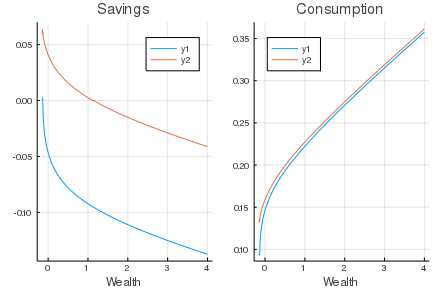
\includegraphics{HuggettPolicies.png} \caption{Policy functions}
\end{figure}

\begin{figure}
\center
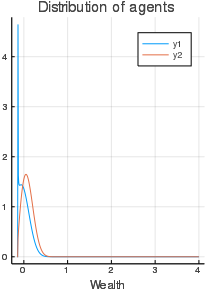
\includegraphics{HuggettDistribution.png} \caption{Distribution}\label{figDist}
\end{figure}

Now, Figure \ref{figDemand} shows the demand curve for bonds for different levels of interest rate. This shows that the function is increasing, so that it crosses any external value of asset supply. In the case of the graph, it is shown that an external supplyof 0 implies an interest rate close to 2\%. Finally, Figure \ref{figShock} shows the response to an unticipated increase in $\lambda_2$. In the long run the interest rate in equilibrium increases, while there is a sharp decrease in the first periods. The stationary distribution shows less agents in the new equilibrium with high income. It can be seen that this is a gradual process.

\begin{figure}
\center
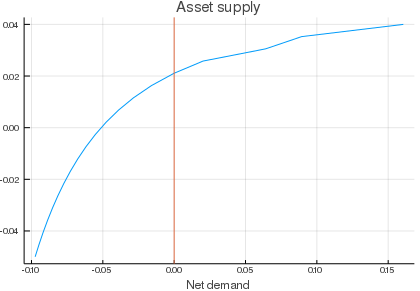
\includegraphics{HuggettSupply.png} \caption{Demand Curve}\label{figDemand}
\end{figure}

\begin{figure}
\center
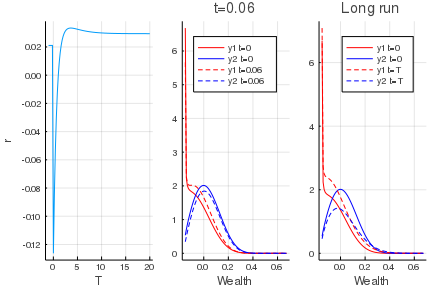
\includegraphics{HuggettShock.png} \caption{Shock to $\lambda_2$ from 0.5 to 0.9}\label{figShock}
\end{figure}

%delta=100, tol=1e-6 rho=0.05 sigma=2 z=0.1,0.2 lambda=0.6,0.5 r=0.03
%shock lambda2 to 0.9

\section{Model with housing}
In this model agents get utility from consumption ($c_t$) and housing ($h_t$), so that their expected utility is $E_0 \int_0^\infty e^{-\rho t}u(c_t,h_t)dt$. Housing can only be consumed in the set $\{0,[h_{min},\infty]\}$. The budget constraint is $\dot{b}_t+p \dot{h}_t=y_t+rb_t-c_t$. In addition, when buying a house the down payment has to be at least a fraction $1-\theta$ of the value of the house ($-b_t\leq \theta p h_t$). The paper focuses on quasi-linear utilities, so that $u(c,h)=\tilde{u}(c+f(h))\equiv \tilde{u}(x)$. So we can write the numerical problem to solve as
\begin{equation}
\begin{split}
&\rho v_j(a) = max_x \tilde{u}(x)+v'_j(a)(y_j+\tilde{f}(a)+ra-x)+\lambda_j(v_{-j}(a)-v_j(a))\\
&\tilde{f}=\max_{h\in \Gamma(a)}(f(h)-rph)
\end{split}
\end{equation}
where $\Gamma(a)=\{h:ph\leq\phi a\}\cap\{0,[h_{min},\infty]\}$

\section{Results for the model with housing}
Now, the model with housing is shown in Figure \ref{figHPol}. There is a decrease in savings up to the point where it is optimal to save in order to buy a house. When wealth is such that optimal housing is higher than $h_{min}$ savings decrease in order to pay for the house. Consumption is decreasing a big part of the state variable because of the savings necessary to achieve the minimum down payment for $h_{min}$. Finally, Figure \ref{figHDist} shows the distribution of agents. There is bunching in the borrowing constraint and above 2.

%delta=1000, tol=1e-6 rho=0.05 sigma=2 z=0.1,0.135 lambda=0.5,0.6 hmin=2.3 p=1, phi=2 alpha=1/3 eta=0.2 utility of housing η*(max(x-hmin,0))^α - r*p*x  r=0.03

\begin{figure}
\center
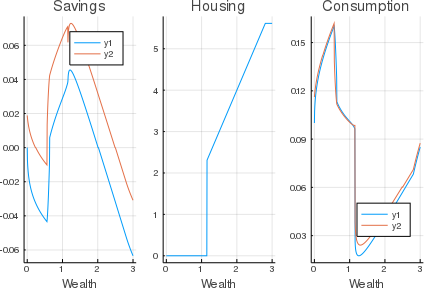
\includegraphics{HousingPolicies.png} \caption{Model with housing. Policy functions}\label{figHPol}
\end{figure}

\begin{figure}
\center
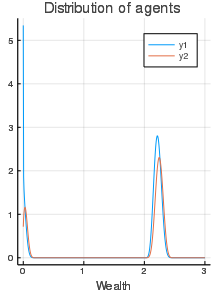
\includegraphics{HousingDistribution.png} \caption{Model with housing. Distribution}\label{figHDist}
\end{figure}



%%%%%%%%%%%%%%%%%%%%%%%%%%%%%%%%%%%%%%

% --------------------------------------------------------------
%     You don't have to mess with anything below this line.
% --------------------------------------------------------------
 
\end{document}